\documentclass[10pt,a4paper]{article}
\usepackage{fontspec}
\usepackage{xeCJK}
\usepackage[margin=18mm]{geometry}
\usepackage{xcolor}
\usepackage{amsmath}
\usepackage{multicol}
\usepackage{tikz}
\setmainfont{Arial}
\setCJKmainfont{SimHei}
\pagestyle{empty}
\setlength{\parindent}{0pt}
\begin{document}
{\fontsize{20}{24}\selectfont\bfseries Layout Analysis Note}\hfill{\small Synthetic Technical Memo 2026}\par
\vspace{2mm}{\color{blue}\rule{\textwidth}{1.8pt}}\par\vspace{4mm}
\begin{multicols}{2}
{\large\bfseries 1. Problem Statement}\par\vspace{2mm}
A two-column page tests reading order. The parser should finish the left column before continuing at the right column. This text deliberately fills a realistic technical paragraph.
\par\vspace{4mm}
{\large\bfseries 2. Formula}\par\vspace{2mm}
Normalized score:
\[
S = \frac{2PR}{P+R}
\]
where $P=0.92$ and $R=0.88$. The expected score is about $0.90$. The equation should remain selectable.
\par\vspace{4mm}
{\large\bfseries 3. Notes}\par\vspace{2mm}
The left column contains the problem, formula, and notes. No OCR is necessary on this page.
\columnbreak
{\large\bfseries 4. Figure}\par\vspace{2mm}
The diagram is a native vector figure and its caption belongs after the diagram.
\begin{center}
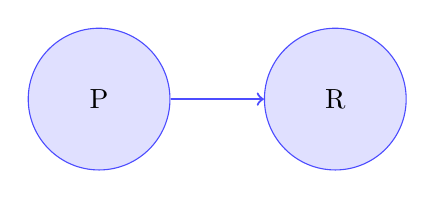
\begin{tikzpicture}
\node[circle,draw=blue!70,fill=blue!12,minimum size=18mm] (p) at (0,0) {P};
\node[circle,draw=blue!70,fill=blue!12,minimum size=18mm] (r) at (3,0) {R};
\draw[->,thick,blue!70] (p) -- (r);
\end{tikzpicture}
\end{center}
\begin{center}\small Figure 1. Precision and recall overlap.\end{center}
\vspace{4mm}
{\large\bfseries 5. Observations}\par\vspace{2mm}
- preserve column order\par
- preserve the equation\par
- keep the caption near Figure 1
\vspace{4mm}
{\large\bfseries 6. Conclusion}\par\vspace{2mm}
Layout evidence is more important than surface-level text completeness.
\end{multicols}
\vfill\scriptsize Synthetic fixture - no personal or customer data\hfill Page 1 of 1
\end{document}